\chapter{A Physics-Constrained Inversion Framework for Ion Energy Flux}
\label{ch:pci}

The preceding chapters established the kinetic and fluid description of the plasma sheath, the forward physics of four optical diagnostics (OES, LIF, Thomson scattering, and interferometry), the machinery of ill-posed inverse problems, and the philosophy of diagnostic fusion. This chapter assembles these into the Physics-Constrained Inversion (PCI) framework: an estimation architecture built on the claim that the ion energy flux $\GammaE$ delivered to a plasma-facing surface, unobservable by any single non-intrusive instrument, is over-determined by the \emph{combination} of four instruments once required to remain consistent with sheath kinetic theory. Reconstructing $\GammaE$ then ceases to be four independent, rank-deficient inversions stitched together and becomes one jointly well-posed nonlinear estimation problem, in which sheath physics supplies the regularization that noisy, incomplete optical data cannot supply alone. The chapter states the problem formally, derives the forward operators, develops the physics constraints as regularizers, solves the regularized objective, extends it to transient and RF-periodic dynamics, describes the numerical pipeline, and closes with the assumptions underlying the construction and their validation.

\section{Formal Statement of the Reconstruction Problem}
\label{sec:pci-formal}

\subsection{Philosophy: estimation rather than sequential deconvolution}

A conventional workflow treats each instrument as a self-contained deconvolution: a Boltzmann plot reduces OES line ratios to $(\ne,\Te)$; an LIF line shape is fitted to a drifting Maxwellian for $\Ti$; a TS spectrum is fitted independently for a second, often inconsistent, $(\ne,\Te)$; an interferometric phase shift is Abel-inverted for $\ne$. Each analysis is individually ill-posed whenever the true distribution departs from the assumed parametric family, and discards covariance information that could correct an earlier estimate. PCI instead poses a single estimation problem over a shared state $\mathbf{m}$ from which all four channels, and $\GammaE$, are computed by explicit, jointly consistent forward operators \cite{ref0711,ref0727} -- the move underlying integrated data analysis (IDA) in magnetic confinement fusion \cite{ref0707,ref0712}, specialized here to the sheath boundary layer, where the regularizing physics is the kinetic and fluid closure of the plasma--sheath transition itself.

\subsection{The unknown state vector}

Let $\mathbf{m}\in\mathbb{R}^{p}$ denote the unknown state of the bulk plasma, presheath, and sheath at a given location and, in the steady formulation of this section, a single instant, partitioned into four blocks:
\begin{align}
\mathbf{m} &= \big(\, \underbrace{\ne,\ \Te,\ \Ti,\ \kappa_{\mathrm e}}_{\text{bulk/presheath moments}}\ ,\ \underbrace{c_{1},\dots,c_{K}}_{\text{IVDF basis coefficients}}\ ,\notag\\
&\qquad \underbrace{V_{0},\ s,\ \gamma_{\mathrm{se}},\ \mathrm{Kn}_{\mathrm i}}_{\text{sheath structure}}\ ,\ \underbrace{\{V_{n},\psi_{n}\}_{n=1}^{N}}_{\text{RF harmonic content (time-resolved case)}} \,\big) \, . \label{eq:state}
\end{align}
$\kappa_{\mathrm e}$ is a shape parameter admitting a controlled departure of the bulk electron energy distribution function (EEDF) from Maxwellian, consistent with the sensitivity of the sheath-formation criterion to non-Maxwellian electrons \cite{ref0090}. The coefficients $c_{1},\dots,c_{K}$ parametrize the ion velocity distribution function (IVDF) $f_{\mathrm i}(v)$ at the sheath edge in a truncated basis (Hermite functions, B-splines, mixture-of-Gaussians):
\begin{equation}
f_{\mathrm i}(v) \;=\; \sum_{k=1}^{K} c_{k}\, \psi_{k}(v)\, , \qquad \int_{-\infty}^{\infty} f_{\mathrm i}(v)\,\mathrm dv = \ni \, . \label{eq:ivdf-basis}
\end{equation}
$V_{0}$ is the time-averaged sheath potential drop, $s$ the sheath thickness, $\gamma_{\mathrm{se}}$ the secondary-electron emission yield, and $\mathrm{Kn}_{\mathrm i}=\lambda_{\mathrm{in}}/s$ the ion Knudsen number controlling the collisionless-to-collisional crossover \cite{ref0077}. The final block, populated only in the time-resolved formulation of \cref{sec:pci-time}, carries the amplitude and phase of the first $N$ harmonics of an RF-driven sheath voltage waveform \cite{ref0043,ref0106}. In practice $p=\dim(\mathbf{m})\sim 10$--$30$, dominated by $K$, kept small relative to the raw data volume so the regularized problem is overdetermined (\cref{sec:pci-overdetermination}).

\subsection{Dimensionality and the design of the state space}

The choice of $p$ is a design decision, not a fixed system property. Too small -- e.g.\ $K=1$, forcing $f_{\mathrm i}(v)$ to a single drifting Maxwellian -- risks biasing the reconstruction whenever the true IVDF carries a resolvable non-Maxwellian feature, such as a double-humped RF-modulated structure or a charge-exchange tail \cite{ref0096}. Too large reintroduces the ill-posedness the framework is built to avoid: extra basis functions $\psi_{k}$ add columns to $\mathbf J$ indistinguishable from noise beyond some order $K^{\star}$, inflating the null space the constraints of \cref{sec:pci-constraints} must suppress. \Cref{sec:pci-algorithm} treats $K$ (and the harmonic order $N$ of \cref{sec:pci-time}) as hyperparameters selected by the same information-theoretic criteria -- residual whiteness, reduced chi-square, cross-validated accuracy -- used to select $\alpha$, rather than fixed a priori.

\subsection{The observable vector and the four forward channels}

The observation vector concatenates the calibrated outputs of the four diagnostics:
\begin{equation}
\mathbf{d} \;=\; \big(\, \mathbf{I}^{\mathrm{OES}} ,\ \mathbf{S}^{\mathrm{LIF}} ,\ \mathbf{S}^{\mathrm{TS}} ,\ \boldsymbol{\Delta\phi}^{\mathrm{INT}} \,\big) \in \mathbb{R}^{q_{1}}\times\mathbb{R}^{q_{2}}\times\mathbb{R}^{q_{3}}\times\mathbb{R}^{q_{4}} , \qquad q=\textstyle\sum_{j} q_{j} \, . \label{eq:data-vector}
\end{equation}
$\mathbf{I}^{\mathrm{OES}}$ is calibrated line intensities at $q_{1}$ wavelengths; $\mathbf{S}^{\mathrm{LIF}}$ the Doppler-resolved fluorescence spectrum at $q_{2}$ detunings; $\mathbf{S}^{\mathrm{TS}}$ the Thomson-scattered power at $q_{3}$ shifts and angles; $\boldsymbol{\Delta\phi}^{\mathrm{INT}}$ the interferometric phase along $q_{4}$ chords. Each block carries its own non-diagonal noise covariance $\boldsymbol{\Sigma}_{j}$, estimated from repeat acquisitions and detector statistics.

\subsection{Operator formalism}

The forward model is the map
\begin{equation}
\mathbf{G}:\ \mathbb{R}^{p}\longrightarrow\mathbb{R}^{q}\, ,\qquad \mathbf{d} = \mathbf{G}(\mathbf{m}) + \boldsymbol{\varepsilon}\, ,\qquad \boldsymbol{\varepsilon}\sim\mathcal N(\mathbf 0,\boldsymbol{\Sigma})\, , \label{ch15-eq:forward-general}
\end{equation}
with $\boldsymbol{\Sigma}=\mathrm{blockdiag}(\boldsymbol{\Sigma}_{1},\boldsymbol{\Sigma}_{2},\boldsymbol{\Sigma}_{3},\boldsymbol{\Sigma}_{4})$ under the testable assumption of uncorrelated cross-instrument noise. $\mathbf{G}$ decomposes into $\mathbf{G}_{\mathrm{OES}},\mathbf{G}_{\mathrm{LIF}},\mathbf{G}_{\mathrm{TS}},\mathbf{G}_{\mathrm{INT}}$ (\cref{sec:pci-forward}), all sharing the argument $\mathbf{m}$. The reconstruction problem is estimation of $\mathbf{m}$, or a posterior over it, from a single realization of $\mathbf{d}$, subject to \cref{sec:pci-constraints}.

\subsection{The target functional}

The reconstruction target is the ion energy flux delivered to the wall,
\begin{equation}
\GammaE \;=\; \frac{1}{2}m_{\mathrm i}\int_{0}^{\infty} v^{3}\, f_{\mathrm i}^{\mathrm{wall}}(v)\,\mathrm dv \, , \label{eq:gammaE-def}
\end{equation}
a nonlinear functional $\GammaE=\mathcal{F}[\mathbf{m}]$ of the wall-directed IVDF obtained by propagating \cref{eq:ivdf-basis} through the sheath transport model, matching energy-flux definitions in the plasma-processing \cite{ref0080,ref0074} and fusion power-balance \cite{ref0093} literature, and collapsing to $\GammaE\approx \Gamma_{\mathrm i}\langle E\rangle_{\mathrm{wall}}$ in the cold-ion limit. Because $\GammaE$ is smooth in $\mathbf{m}$, its uncertainty follows from propagating the covariance of $\hat{\mathbf{m}}$ through the linearization of $\mathcal{F}$ (\cref{sec:pci-algorithm}).

\section{The Forward Model: From Sheath Kinetics to Four Optical Observables}
\label{sec:pci-forward}

\subsection{The presheath--sheath kinetic sub-model}

The forward operators draw on a common kinetic/fluid sub-model. The sheath-edge ion flux is fixed by the generalized kinetic Bohm criterion,
\begin{equation}
\int_{-\infty}^{\infty} \frac{f_{\mathrm i}(v)}{v^{2}}\,\mathrm dv \;\le\; \frac{n_{\mathrm s}}{e\Te}\, , \label{eq:bohm-kinetic}
\end{equation}
which collapses, for a mono-energetic or drifting-Maxwellian population, to $u_{i,\mathrm s}\ge\uB=\sqrt{e\Te/m_{\mathrm i}}$ in the cold-fluid limit. Within the sheath the ions are collisionless (or weakly collisional, via $\mathrm{Kn}_{\mathrm i}$) and fall through the self-consistent potential governed by Poisson's equation,
\begin{equation}
\varepsilon_{0}\frac{\mathrm d^{2}\phi}{\mathrm dx^{2}} = e\big(\ne(x)-\ni(x)\big)\, ,\qquad \phi(0)=0,\ \ \phi(s)=-V_{0}\, , \label{eq:poisson-sheath}
\end{equation}
with ions obeying $\tfrac12 m_{\mathrm i}v(x)^{2} = \tfrac12 m_{\mathrm i}v_{\mathrm s}^{2} + e[\phi(0)-\phi(x)]$ and $\ni(x)v(x)=n_{\mathrm s}u_{\mathrm i,s}$ per velocity class. Solving \cref{eq:poisson-sheath} self-consistently advances $f_{\mathrm i}(v)$ to a wall-arrival distribution $f_{\mathrm i}^{\mathrm{wall}}(v)$ \cite{ref0083,ref0672}. This propagation operator, $\mathcal T_{\mathrm{sheath}}[\,\cdot\,;V_{0},s,\mathrm{Kn}_{\mathrm i}]$, links the sheath-edge state (probed by LIF and TS) to the wall, where $\GammaE$ is defined and direct-flux sensors provide independent calibration \cite{ref0075}.

\subsection{OES forward operator}

OES measures line-integrated photon emission from levels populated, in a low-temperature optically thin plasma, predominantly by electron-impact excitation and cascade. Writing $X_{jk}(\ne,\Te,\kappa_{\mathrm e})$ for the effective population coefficient of transition $j\!\to\! k$ (from a collisional--radiative balance sensitive to the EEDF shape when $\kappa_{\mathrm e}\ne1$), the predicted line intensity along a chord of length $\ell$ is
\begin{equation}
I^{\mathrm{OES}}_{jk}[\mathbf m] \;=\; \frac{A_{jk}}{4\pi}\int_{0}^{\ell} \ne(x)\, n_{0}(x)\, X_{jk}\big(\ne(x),\Te(x),\kappa_{\mathrm e}\big)\,\mathrm dx \, , \label{eq:G-oes}
\end{equation}
with $A_{jk}$ the Einstein coefficient and $n_{0}$ the feeding-level density, known from gas pressure and ionization fraction. Ratios of lines with different excitation thresholds fix $\Te$ largely independent of absolute calibration, exploited to fix $(\ne,\Te,\kappa_{\mathrm e})$ jointly via a collisional--radiative model \cite{ref0275}. $\mathbf G_{\mathrm{OES}}(\mathbf m)$ stacks \cref{eq:G-oes} over the $q_{1}$ observed lines.

\subsection{LIF forward operator}

LIF probes the IVDF directly via the Doppler shift of a resonant absorption line. The fluorescence signal at detuning $\nu$ is the ion distribution convolved with the combined laser and natural line shape $\mathcal L$,
\begin{equation}
S^{\mathrm{LIF}}[\mathbf m](\nu) \;=\; \eta_{\mathrm{LIF}}\int_{-\infty}^{\infty} f_{\mathrm i}(v)\, \mathcal L\!\left(\nu-\nu_{0}\Big(1+\frac{v}{c}\Big)\right)\mathrm dv \, , \label{eq:G-lif}
\end{equation}
with $\eta_{\mathrm{LIF}}$ a calibrated instrumental efficiency. Because $f_{\mathrm i}(v)$ enters linearly through a convolution, LIF is the channel most informative about the shape coefficients $c_{1},\dots,c_{K}$; its single-diagnostic inversion is correspondingly ill-conditioned, since deconvolving $\mathcal L$ amplifies high-frequency noise -- the setting in which Tikhonov-type regularization of distribution-function reconstructions was developed, e.g.\ for tomographic absorption spectroscopy \cite{ref0677}.

\subsection{Thomson scattering forward operator}

TS measures spectral power scattered from free electrons, resolved in wavelength shift $\Delta\lambda$ at fixed angle $\theta$. In the collective regime relevant to most low-temperature plasmas, the scattered spectrum is proportional to the dynamic form factor $S(k,\omega)$,
\begin{equation}
S^{\mathrm{TS}}[\mathbf m](\Delta\lambda,\theta) \;=\; \eta_{\mathrm{TS}}\, \ne\, S\!\big(k,\omega;\Te,\kappa_{\mathrm e},\Ti\big) \, ,\qquad k = \frac{4\pi}{\lambda_{0}}\sin\!\frac{\theta}{2} \, , \label{eq:G-ts}
\end{equation}
with $\omega=2\pi c\,\Delta\lambda/\lambda_{0}^{2}$. $S(k,\omega)$ carries an electron feature whose width fixes $\Te$ and whose non-Gaussianity is sensitive to $\kappa_{\mathrm e}$, and, at low $k\lD$, an ion-acoustic feature sensitive to $\Ti/\Te$. TS is thus the primary, least model-dependent source of an independent $\Te$ cross-check against OES, a role it also plays in tokamak diagnostics \cite{ref0683,ref0684}.

\subsection{Interferometry forward operator}

Interferometry measures the phase shift accumulated along a probe chord, proportional to line-integrated electron density,
\begin{equation}
\Delta\phi^{\mathrm{INT}}[\mathbf m](y) \;=\; \frac{e^{2}}{2\varepsilon_{0} m_{\mathrm e} c\,\omega_{\mathrm{probe}}}\int_{-\infty}^{\infty} \ne(x,y)\,\mathrm dx \, , \label{eq:G-int}
\end{equation}
for chords indexed by impact parameter $y$. Since this is a Radon-type projection, recovering spatially resolved $\ne(x,y)$ requires an Abel or tomographic inversion whenever the column is non-uniform \cite{ref0399}; this preprocessing is folded into $\mathbf G_{\mathrm{INT}}$, so the interferometric datum entering the misfit is the calibrated chord phase.

\subsection{The composite forward map and its sensitivity structure}

Stacking \cref{eq:G-oes,eq:G-lif,eq:G-ts,eq:G-int} gives $\mathbf G(\mathbf m)$, with local sensitivity given by the block Jacobian
\begin{equation}
\mathbf J(\mathbf m) = \frac{\partial \mathbf G}{\partial \mathbf m} = \begin{pmatrix} \partial \mathbf G_{\mathrm{OES}}/\partial \mathbf m \\ \partial \mathbf G_{\mathrm{LIF}}/\partial \mathbf m \\ \partial \mathbf G_{\mathrm{TS}}/\partial \mathbf m \\ \partial \mathbf G_{\mathrm{INT}}/\partial \mathbf m \end{pmatrix} \in \mathbb R^{q\times p} \, , \label{ch15-eq:jacobian}
\end{equation}
whose row blocks have complementary sparsity (\cref{tab:forward-summary}): $\mathbf G_{\mathrm{OES}},\mathbf G_{\mathrm{TS}}$ are most sensitive to $(\ne,\Te,\kappa_{\mathrm e})$ and only weakly to $c_{k}$; $\mathbf G_{\mathrm{LIF}}$ is most sensitive to $c_{k}$ and only weakly to $\ne$; $\mathbf G_{\mathrm{INT}}$ senses only chord-integrated $\ne$. No single block has full column rank, so any one channel's inversion is ill-posed; but the four null spaces intersect only along directions consistent with \cref{sec:pci-constraints}, so the stacked problem can be made well-posed.

Evaluating $\mathbf J(\mathbf m)$ at each Gauss--Newton step (\cref{sec:pci-objective}) is dominated by two operators requiring a nested physics solve -- $\mathbf G_{\mathrm{OES}}$ (a re-solved collisional--radiative balance) and $\mathcal T_{\mathrm{sheath}}$ inside $C_{3},C_{4}$ -- both amenable to automatic differentiation and to the surrogate-acceleration strategy of \cref{sec:pci-algorithm}.

\begin{table}[htbp]
\centering
\caption{Summary of the four forward operators comprising the composite map $\mathbf G(\mathbf m)$: nominal sensitivity to each block of the state vector (H = high, M = moderate, L = low/negligible).}
\label{tab:forward-summary}
\begin{tabularx}{\textwidth}{@{}l l c c c c@{}}
\toprule
Channel & Governing equation & $(\ne,\Te,\kappa_{\mathrm e})$ & $\Ti$ & IVDF shape $c_{k}$ & Sheath geometry $(V_{0},s)$ \\
\midrule
OES & \cref{eq:G-oes} & H & L & L & L \\
LIF & \cref{eq:G-lif} & L & H & H & M \\
Thomson scattering & \cref{eq:G-ts} & H & M & L & L \\
Interferometry & \cref{eq:G-int} & M ($\ne$ only) & L & L & L \\
\bottomrule
\end{tabularx}
\end{table}

\section{Physics Constraints as Regularizers}
\label{sec:pci-constraints}

\subsection{The role of constraints in an ill-posed problem}

\Cref{tab:forward-summary} shows the raw, unconstrained least-squares problem $\min_{\mathbf m}\|\mathbf W(\mathbf G(\mathbf m)-\mathbf d)\|_{2}^{2}$ is ill-conditioned: $\mathbf J^{\mathsf T}\mathbf J$ has small or vanishing eigenvalues along directions that change IVDF shape without changing any predicted data block (e.g.\ redistributing $f_{\mathrm i}(v)$ among $\psi_{k}$ while conserving the moments each instrument senses). A generic smoothness or minimum-norm penalty (\cref{sec:pci-objective}) is not the most informative regularizer here, since the sheath obeys known conservation laws and boundary conditions that constrain physically admissible directions far more tightly than a generic prior \cite{ref0692}. PCI therefore promotes six physics relations from post-hoc checks to regularizing constraints imposed \emph{during} estimation.

\subsection{C1 -- The kinetic Bohm criterion}

The sheath-edge state must satisfy \cref{eq:bohm-kinetic}, recast as a constraint residual,
\begin{equation}
C_{1}(\mathbf m) \;=\; \int_{-\infty}^{\infty}\frac{f_{\mathrm i}(v)}{v^{2}}\,\mathrm dv \;-\; \frac{n_{\mathrm s}}{e\Te} \;\le\; 0 \, . \label{eq:C1}
\end{equation}
Being an inequality, it is implemented as a one-sided penalty, preventing the optimizer from drifting into an IVDF that could not sustain a stationary sheath -- a failure mode unconstrained fits of non-Maxwellian IEDFs are prone to \cite{ref0090,ref0096}.

\subsection{C2 -- Sheath electrostatics (generalized Poisson/Child--Langmuir)}

$V_{0}$, $s$, and $n_{\mathrm s}u_{\mathrm i,s}$ are linked by the integrated form of \cref{eq:poisson-sheath}, which in the collisionless, cold-ion, high-voltage limit reduces to Child--Langmuir,
\begin{equation}
n_{\mathrm s}u_{\mathrm i,s} \;=\; \frac{4}{9}\varepsilon_{0}\sqrt{\frac{2}{e\,m_{\mathrm i}}}\,\frac{V_{0}^{3/2}}{s^{2}} \, , \label{ch15-eq:child-langmuir}
\end{equation}
and more generally to the full boundary-value problem \cref{eq:poisson-sheath}. $C_{2}(\mathbf m)$ is the deviation of $(V_{0},s,n_{\mathrm s}u_{\mathrm i,s})$ from this manifold (or its collisional generalization when $\mathrm{Kn}_{\mathrm i}\lesssim 1$ \cite{ref0077}), letting a sheath thickness inferred indirectly from an RF harmonic amplitude \cite{ref0043} discipline the flux normalization used by LIF and OES.

\subsection{C3 -- Particle-flux continuity}

With negligible ionization inside the thin collisionless sheath, ion particle flux is conserved from sheath edge to wall:
\begin{equation}
C_{3}(\mathbf m) \;=\; n_{\mathrm s}u_{\mathrm i,s} \;-\; \int_{0}^{\infty} v\, f_{\mathrm i}^{\mathrm{wall}}(v)\,\mathrm dv \;=\; 0 \, , \label{eq:C3}
\end{equation}
with $f_{\mathrm i}^{\mathrm{wall}}$ from $\mathcal T_{\mathrm{sheath}}$. This ties the LIF-sensitive IVDF shape directly to the wall-arrival flux in \cref{eq:gammaE-def}, making $\GammaE$ estimable from sheath-edge, rather than wall-embedded, diagnostics \cite{ref0119}.

\subsection{C4 -- Energy-flux and power-balance consistency}

A companion constraint enforces consistency between the energy carried by $f_{\mathrm i}^{\mathrm{wall}}$ and the budget implied by bulk parameters and the sheath energy-transmission coefficient $\langle E\rangle_{\mathrm{wall}}/\Te$ (a function of $V_{0}/\Te$, $\gamma_{\mathrm{se}}$, and $\Ti/\Te$):
\begin{equation}
C_{4}(\mathbf m) \;=\; \GammaE^{\mathrm{(kinetic)}} \;-\; \Gamma_{\mathrm i}\big[\,e V_{0} + \varsigma\,\Te\, \big] \;=\; 0 \, , \label{eq:C4}
\end{equation}
where $\varsigma$ is an $O(1)$ fluid-closure coefficient. This is the sheath-scale analogue of power-balance constraints for plasma-facing-surface energy budgets \cite{ref0093,ref0080}, most sensitive to $\gamma_{\mathrm{se}}$ -- why $\gamma_{\mathrm{se}}$ is retained as an explicit unknown in \cref{eq:state} rather than fixed a priori.

\subsection{C5 -- Fluid--kinetic moment closure}

The zeroth and second moments of $f_{\mathrm i}(v)$ must agree, within uncertainty, with the fluid quantities $\ni\approx\ne$ and $\Ti$ from interferometric/OES density and the LIF or TS ion-feature width:
\begin{equation}
C_{5,0}(\mathbf m) = \int f_{\mathrm i}\,\mathrm dv - \ni\, ,\qquad C_{5,2}(\mathbf m) = m_{\mathrm i}\!\int (v-\bar v)^{2} f_{\mathrm i}\,\mathrm dv - \ni e\Ti \, . \label{eq:C5}
\end{equation}
This is a direct instance of the kinetic/fluid moment-closure check discussed for heat-flux-carrying sheaths \cite{ref0101}: the mechanism by which OES/interferometry-derived $\ne$ disciplines the amplitude, not shape, of the LIF-derived $f_{\mathrm i}(v)$.

\subsection{C6 -- Smoothness and maximum-entropy priors on the IVDF}

Even after C1--C5, high-order coefficients $c_{k}$ may remain invisible to all four channels within the noise floor. These are controlled by a maximum-entropy or total-variation penalty,
\begin{equation}
R_{\mathrm{ent}}(\mathbf m) = -\int f_{\mathrm i}(v)\ln\!\frac{f_{\mathrm i}(v)}{f_{\mathrm i}^{\mathrm{ref}}(v)}\,\mathrm dv \, ,\quad\text{or}\quad R_{\mathrm{TV}}(\mathbf m) = \int \left|\frac{\mathrm d f_{\mathrm i}}{\mathrm dv}\right|\mathrm dv \, , \label{eq:C6}
\end{equation}
with $f_{\mathrm i}^{\mathrm{ref}}$ a weakly informative reference (a Maxwellian at fluid $\Ti$), following a long history of such regularization in spectroscopic inverse problems \cite{ref0677}. Total-variation is preferred whenever the IVDF retains sharp features an entropy penalty would over-smooth \cite{ref0692}; the choice and weight is a model-selection decision informed by \cref{sec:pci-algorithm}.

\subsection{Hard versus soft enforcement}

C1--C6 are not enforced identically. Constraints whose physical uncertainty is negligible against optical noise -- chiefly C2 and C3, following from conservation with essentially no free parameters once collisionality is fixed -- are eliminated exactly via the Lagrangian of \cref{sec:pci-objective}. Constraints whose right-hand side carries non-trivial physical uncertainty, such as C4 (through $\gamma_{\mathrm{se}}$) and C5 (fluid-side moments are themselves estimates), are retained as soft, quadratically penalized residuals whose weight $\mu_{j}$ is set by the estimated variance of the physical law, letting the optimizer trade a small violation for a better data fit exactly as much as the physics justifies. This avoids over-constraining the problem: treating every relation as exact would simply relocate the ill-posedness into an inconsistent constraint system.

\subsection{Over-determination from complementary diagnostics}
\label{sec:pci-overdetermination}

\Cref{tab:constraint-summary} tallies constraints against state dimension. With $p\sim 10$--$30$ unknowns, six constraint families (C1 inequality-type, not reducing degrees of freedom unless active), and $q$ typically hundreds to low thousands of raw samples, the composite, constrained problem is over-determined: $\mathrm{rank}\big[\mathbf J^{\mathsf T}\mathbf J + \sum_{j}\mu_{j}\,(\partial C_{j}/\partial\mathbf m)^{\mathsf T}(\partial C_{j}/\partial\mathbf m)\big] = p$ can be certified numerically at convergence (\cref{sec:pci-algorithm}). This is the multi-instrument analogue of the redundancy exploited by Bayesian multi-diagnostic inference at tokamak divertors \cite{ref0685} and joint inference of Hall-thruster plasmas \cite{ref0719}: each additional channel adds rows to $\mathbf J$ whose null space generically does not coincide with that of the others, so the intersection of all null spaces shrinks with each diagnostic added and vanishes once the physics constraints are included.

\begin{table}[htbp]
\centering
\caption{Physics constraints used as regularizers in the PCI objective, their type, and the principal quantities they couple across the four observable channels.}
\label{tab:constraint-summary}
\begin{tabularx}{\textwidth}{@{}c l l X@{}}
\toprule
ID & Physics & Type & Principal channels linked \\
\midrule
C1 & Kinetic Bohm criterion (\cref{eq:C1}) & Inequality & LIF (IVDF shape) $\leftrightarrow$ OES/TS ($\Te$) \\
C2 & Sheath electrostatics (\cref{ch15-eq:child-langmuir}) & Equality & RF waveform $\leftrightarrow$ LIF flux normalization \\
C3 & Particle-flux continuity (\cref{eq:C3}) & Equality & LIF $\leftrightarrow$ $\GammaE$ target \\
C4 & Energy/power-balance consistency (\cref{eq:C4}) & Equality & LIF, OES/TS $\leftrightarrow$ $\GammaE$ target \\
C5 & Fluid--kinetic moment closure (\cref{eq:C5}) & Equality (soft) & LIF $\leftrightarrow$ OES/TS/INT \\
C6 & IVDF smoothness/entropy (\cref{eq:C6}) & Penalty & LIF null space only \\
\bottomrule
\end{tabularx}
\end{table}

\section{The Regularized Objective and Its Solution}
\label{sec:pci-objective}

\subsection{Composite objective functional}

Collecting the weighted data misfit, the Tikhonov term, and the physics-constraint penalties gives
\begin{align}
J(\mathbf m) \;=\; &\underbrace{\tfrac12\big\|\boldsymbol{\Sigma}^{-1/2}\big(\mathbf G(\mathbf m)-\mathbf d\big)\big\|_{2}^{2}}_{\text{data misfit}} \;+\; \underbrace{\tfrac{\alpha}{2}\big\|\mathbf L(\mathbf m-\mathbf m_{\mathrm{ref}})\big\|_{2}^{2}}_{\text{Tikhonov prior}} \notag \\
&+\; \underbrace{\beta\, R_{\mathrm{ent/TV}}(\mathbf m)}_{\text{C6}} \;+\; \underbrace{\sum_{j=2}^{5}\frac{\mu_{j}}{2}\, C_{j}(\mathbf m)^{2}}_{\text{soft equality constraints}} \;+\; \underbrace{\mu_{1}\big[\max(0,C_{1}(\mathbf m))\big]^{2}}_{\text{C1}} \, , \label{eq:objective}
\end{align}
where $\mathbf L$ is a block-diagonal smoothness operator, $\mathbf m_{\mathrm{ref}}$ a weakly informative prior mean (the single-diagnostic estimates of \cref{sec:pci-algorithm}), and $\alpha,\beta,\{\mu_{j}\}$ regularization weights: $\alpha$ set by the L-curve/discrepancy procedure of \cref{sec:pci-algorithm}, and $\mu_{j}$ either fixed large enough to enforce near-exact satisfaction of C2--C4, or treated as inverse-variance hyperparameters and marginalized in a Bayesian reading. The two readings of \cref{eq:objective} -- penalized least squares, or minus the log-posterior of a Bayesian model whose MAP coincides with the minimizer -- are used interchangeably below, following established Bayesian-IDA practice \cite{ref0707,ref0709,ref0710}.

\subsection{Stationarity and the Lagrangian view}

Where a constraint is instead imposed exactly (C2, C3), the term is removed from the penalty sum and enforced via a Lagrange multiplier $\boldsymbol\lambda$:
\begin{equation}
\mathcal L(\mathbf m,\boldsymbol\lambda) = J_{\mathrm{unconstrained}}(\mathbf m) + \boldsymbol\lambda^{\mathsf T}\mathbf C_{\mathrm{hard}}(\mathbf m) \, , \label{eq:lagrangian}
\end{equation}
whose Karush--Kuhn--Tucker conditions,
\begin{align}
\nabla_{\mathbf m} J_{\mathrm{unconstrained}}(\mathbf m^{\star}) + \left(\frac{\partial \mathbf C_{\mathrm{hard}}}{\partial \mathbf m}\right)^{\!\mathsf T}\!\boldsymbol\lambda^{\star} &= \mathbf 0 \, , \label{eq:kkt1}\\
\mathbf C_{\mathrm{hard}}(\mathbf m^{\star}) &= \mathbf 0 \, , \label{eq:kkt2}
\end{align}
define $\mathbf m^{\star}$: the point on $\{\mathbf m:\mathbf C_{\mathrm{hard}}(\mathbf m)=\mathbf 0\}$ closest, in the metric induced by $\boldsymbol\Sigma^{-1}$ and $\mathbf L$, to reproducing $\mathbf d$.

\subsection{Gauss--Newton / Levenberg--Marquardt solution}

Because $\mathbf G$ and $\mathbf C_{\mathrm{hard}}$ are nonlinear in $\mathbf m$, \cref{eq:objective} is minimized iteratively: linearizing about $\mathbf m_{k}$, $\mathbf G(\mathbf m)\approx \mathbf G(\mathbf m_{k})+\mathbf J_{k}(\mathbf m-\mathbf m_{k})$, and forming the Gauss--Newton normal equations for $\Delta\mathbf m_{k}=\mathbf m_{k+1}-\mathbf m_{k}$,
\begin{equation}
\Big[\mathbf J_{k}^{\mathsf T}\boldsymbol\Sigma^{-1}\mathbf J_{k} + \alpha\,\mathbf L^{\mathsf T}\mathbf L + \sum_{j}\mu_{j}\big(\mathbf D_{j,k}\big)^{\mathsf T}\mathbf D_{j,k} + \eta_{k}\mathbf I\Big]\Delta\mathbf m_{k} = -\,\mathbf g_{k} \, , \label{eq:gauss-newton}
\end{equation}
with $\mathbf g_{k}$ the gradient at $\mathbf m_{k}$, $\mathbf D_{j,k}=\partial C_{j}/\partial\mathbf m|_{\mathbf m_{k}}$, and $\eta_{k}\ge 0$ a Levenberg--Marquardt damping coefficient adapted trust-region-style. This is the normal-equation structure common to Tikhonov-regularized inverse problems \cite{ref0695}, specialized by the physics-constraint Gram terms $\mathbf D_{j,k}^{\mathsf T}\mathbf D_{j,k}$, which raise the smallest eigenvalues of the bracketed matrix above the noise floor that would otherwise leave it numerically singular.

\subsection{Well-posedness}

Well-posedness in the Hadamard sense requires existence, uniqueness, and stability. \emph{Existence} follows from the direct method of the calculus of variations: $J$ is continuous, bounded below, and coercive once the Tikhonov and entropy/TV terms are active, guaranteeing a minimizer by the weak-lower-semicontinuity argument used for Tikhonov-type functionals \cite{ref0692}. \emph{Uniqueness} is unavailable for the unconstrained data term alone (the null-space argument of \cref{sec:pci-overdetermination}), but is restored locally once the Gram matrix in \cref{eq:gauss-newton} is positive definite -- verified numerically via its smallest eigenvalue, guaranteed whenever the four channel null spaces intersect the tangent space of $\{\mathbf C_{\mathrm{hard}}=\mathbf 0\}$ only trivially. \emph{Stability} follows from a variational source condition: reconstruction error is bounded by a constant multiple of the data-noise level, degrading gracefully as $\alpha\to 0$, unlike the unconstrained problem, whose stability constant is unbounded along the shared null space.

This is certified numerically at every converged solution by inspecting the smallest eigenvalue of the bracketed Gram matrix and its eigenvector. An eigenvalue well above the noise floor, aligned with no single physically meaningful direction, evidences that over-determination has been realized for the dataset at hand; a small eigenvalue aligned with a specific $c_{k}$ or a weakly excited harmonic $V_{n}$ flags that an additional measurement or tighter prior is needed before that component of $\hat{\mathbf m}$, and hence $\hat\Gamma_{E}$, can be trusted, and is reported alongside $\hat\Gamma_{E}$ as standard pipeline output (\cref{sec:pci-algorithm}).

\section{Time-Resolved Formulation for Transient Sheath Dynamics}
\label{sec:pci-time}

\subsection{Motivation}

Sections~\ref{sec:pci-formal}--\ref{sec:pci-objective} treat $\mathbf m$ as time-independent, appropriate for a DC or slowly varying discharge. Many technologically important sheaths are strongly modulated: RF sheaths oscillate at the drive frequency and harmonics (typically \SI{13.56}{\mega\hertz} industrially) with a voltage swing that can exceed the time-averaged drop by an order of magnitude \cite{ref0043}, ion-implantation sheaths expand and collapse on \SI{1}{\micro\second} timescales under a pulsed bias, and electrical-asymmetry-effect sources impose a slow, tailorable modulation on the fast RF cycle \cite{ref0106}. In these cases the target is a time-resolved $\GammaE(t)$, not the single $\GammaE$ of \cref{eq:gammaE-def}; a static inversion of time-averaged data would systematically bias the reconstructed IVDF shape whenever the sheath response is nonlinear in the drive -- which it always is, at the level of the Child--Langmuir scaling \cref{ch15-eq:child-langmuir}.

\subsection{A representative scenario}

In a capacitively coupled discharge with an added low-frequency bias, as in an electrical-asymmetry-effect source \cite{ref0106}, a static reconstruction would return a single $\hat\Gamma_{E}$ mixing contributions from the entire range of instantaneous sheath voltages, including the brief high-voltage portion disproportionately responsible for sputtering. The time-resolved formulation instead returns $\hat\Gamma_{E}(\theta)$ across the drive cycle, from the same four channels with no additional hardware beyond phase-locking (\cref{eq:phase-forward}).

\subsection{State-space augmentation}

The formulation augments \cref{eq:state} with its anticipated harmonic block, treating the full state as a function of RF phase $\theta=\omega t\ \mathrm{mod}\ 2\pi$ (periodic case) or time $t$ directly (aperiodic transient):
\begin{equation}
\mathbf m(\theta) \;=\; \mathbf m_{0} \;+\; \sum_{n=1}^{N} \Big[\mathbf m_{n}^{c}\cos(n\theta) + \mathbf m_{n}^{s}\sin(n\theta)\Big] \, , \label{eq:fourier-state}
\end{equation}
a truncated Fourier representation automatically enforcing $\mathbf m(0)=\mathbf m(2\pi)$, with truncation order $N$ chosen, like $K$, by the convergence diagnostics of \cref{sec:pci-algorithm}. For aperiodic transients, \cref{eq:fourier-state} is replaced by a piecewise representation on a time grid, periodicity replaced by an explicit temporal-smoothness penalty (\cref{sec:pci-time-reg}).

\subsection{Phase-resolved and phase-blind data}

The four channels are not equally capable of resolving $\theta$. Pulsed-laser diagnostics -- LIF and, with a pulsed probe, TS -- can be phase-locked and gated to record $\mathbf S^{\mathrm{LIF}}(\nu;\theta_{i})$ and $\mathbf S^{\mathrm{TS}}(\Delta\lambda;\theta_{i})$ at discrete bins $\{\theta_{i}\}$, as can phase-resolved OES with a fast-gated camera, whereas continuous-wave interferometry integrates over many RF periods and delivers only $\langle\ne\rangle$, constraining $\mathbf m_{0}$ but not $\mathbf m_{n}^{c},\mathbf m_{n}^{s}$ for $n\ge 1$. The time-resolved forward operators are accordingly
\begin{equation}
\mathbf d(\theta_{i}) = \mathbf G\big(\mathbf m(\theta_{i})\big) + \boldsymbol\varepsilon_{i}\quad (\text{LIF, TS, phase-resolved OES})\, ,\qquad \bar{\mathbf d}^{\mathrm{INT}} = \mathbf G_{\mathrm{INT}}\Big(\frac{1}{2\pi}\!\int_{0}^{2\pi}\!\mathbf m(\theta)\,\mathrm d\theta\Big) + \bar{\boldsymbol\varepsilon} \, , \label{eq:phase-forward}
\end{equation}
and the time-resolved objective sums the phase-resolved misfit over $\{\theta_{i}\}$ plus the cycle-averaged interferometric term, which stabilizes $\mathbf m_{0}$ while harmonic content is resolved by the genuinely time-resolved channels \cite{ref0043,ref0106}.

\subsection{Temporal regularization}
\label{sec:pci-time-reg}

C1--C6 are applied pointwise at every $\theta_{i}$ (the Bohm criterion and electrostatics must hold instantaneously, not merely on cycle average), supplemented by a temporal-smoothness penalty discouraging phase-to-phase oscillation unsupported by the harmonic truncation,
\begin{equation}
R_{\mathrm{time}}(\mathbf m) \;=\; \frac{\gamma}{2}\int_{0}^{2\pi} \left\|\frac{\mathrm d^{2}\mathbf m}{\mathrm d\theta^{2}}\right\|_{2}^{2}\mathrm d\theta \, . \label{eq:temporal-reg}
\end{equation}
Where the transient has a genuine discontinuity (a step bias at $t=0$), a total-variation-in-time penalty is substituted, exactly as C6 substitutes $R_{\mathrm{TV}}$ for $R_{\mathrm{ent}}$ when a sharp IVDF feature is expected.

\subsection{Global versus sequential estimation}

Two strategies solve the augmented problem. The \emph{global} strategy stacks all phase bins into one Gauss--Newton system \cref{eq:gauss-newton}, with $\mathbf m$ replaced by the Fourier coefficients of \cref{eq:fourier-state}; most statistically efficient, yielding a single self-consistent posterior covariance over the full waveform, but scaling as $O\big((Np)^{3}\big)$ per step. The \emph{sequential} strategy propagates a phase-to-phase estimate, updating a running state and covariance as each bin's data arrives, in the spirit of a nonlinear, constrained Kalman filter; cheaper per step and the natural choice for near-real-time monitoring, particularly once accelerated by a trained surrogate \cite{ref0728,ref0731}. Both target the same posterior implied by \cref{eq:objective,eq:temporal-reg}, and the sequential estimate can be refined by a final global pass.

\section{Algorithm, Workflow, and Data Pipeline}
\label{sec:pci-algorithm}

\subsection{Overview}

\Cref{fig:pci-pipeline} sketches the data flow from the four raw diagnostic streams to the final estimate of $\GammaE$ (or $\GammaE(\theta)$) with credible interval. The workflow comprises six stages, each with an explicit acceptance criterion: because $\hat\Gamma_{E}$ is several nonlinear transformations removed from any raw measurement, a user needs visibility into calibration curves, initial estimates, regularization-parameter selection, and constraint residuals to distinguish a trustworthy reconstruction from an overfit or under-constrained one.

\begin{figure}[htbp]
\centering
\begin{tikzpicture}[
 box/.style={draw, thick, text width=2.3cm, minimum height=1.05cm, align=center, font=\scriptsize, inner sep=3pt},
 arr/.style={-{Latex[length=2.2mm]}, thick}
]
\node[box] (oes) at (0,3.3) {OES\\line ratios};
\node[box] (lif) at (0,1.1) {LIF\\Doppler spectra};
\node[box] (ts) at (0,-1.1) {Thomson\\scattering};
\node[box] (int) at (0,-3.3) {Interferometry\\phase};
\node[box, text width=2.4cm, minimum height=3.6cm] (fwd) at (3.4,0) {Forward operators\\$\mathbf G_{\mathrm{OES}},\mathbf G_{\mathrm{LIF}}$\\$\mathbf G_{\mathrm{TS}},\mathbf G_{\mathrm{INT}}$};
\node[box, minimum height=1.6cm] (obj) at (6.9,1.4) {Regularized\\objective\\$J(\mathbf m)$};
\node[box, minimum height=1.6cm] (phys) at (6.9,-1.9) {Physics\\constraints\\C1--C6};
\node[box] (opt) at (10.3,0) {Constrained\\Gauss--Newton\\optimizer};
\node[box] (state) at (13.7,1.4) {State $\hat{\mathbf m}$:\\$\hat n_{\mathrm e},\hat T_{\mathrm e},\hat T_{\mathrm i},$\\$\hat f_{\mathrm i}(v),\ldots$};
\node[box] (out) at (13.7,-1.9) {$\hat\Gamma_{E}$ + credible\\interval};
\draw[arr] (oes) -- (fwd.west |- oes);
\draw[arr] (lif) -- (fwd.west |- lif);
\draw[arr] (ts) -- (fwd.west |- ts);
\draw[arr] (int) -- (fwd.west |- int);
\draw[arr] (fwd) -- (obj);
\draw[arr] (phys) -- (obj);
\draw[arr] (obj) -- (opt.north -| obj) -- (opt);
\draw[arr] (opt) -- (state);
\draw[arr] (opt) -- (out);
\end{tikzpicture}
\caption{Schematic (illustrative, not to scale) data flow of the physics-constrained inversion pipeline. Four calibrated optical data streams enter shared forward operators; the resulting predictions are combined with the sheath physics constraints C1--C6 into a single regularized objective, minimized by a constrained Gauss--Newton iteration to yield the joint state estimate $\hat{\mathbf m}$ and the derived ion energy flux $\hat\Gamma_{E}$ with its propagated uncertainty. The diagram is a structural sketch of the algorithm, not a rendering of any measured dataset.}
\label{fig:pci-pipeline}
\end{figure}

\subsection{Stage 1 -- Synchronized acquisition}

The four instruments share a common timebase (phase-locked to the RF drive for the time-resolved formulation), and each acquisition is tagged with timestamp, integration window, and instrument state, so instrument-specific systematics can be modelled explicitly in $\mathbf G$ rather than absorbed into unstructured noise.

\subsection{Stage 2 -- Preprocessing and calibration}

Raw detector output is reduced to calibrated units: OES background-subtracted and instrument-response corrected; LIF corrected for laser power drift and saturation; TS stray-light-subtracted; interferometric phase unwrapped and, where non-uniform, Abel-inverted with a regularized tomographic technique \cite{ref0417}. Each step propagates its own uncertainty into $\boldsymbol\Sigma_{j}$ rather than being treated as exact.

\subsection{Stage 3 -- Initialization from single-diagnostic analytic inversions}

A deliberately crude estimate $\mathbf m^{(0)}$ is formed from the classical analyses -- a Boltzmann-plot $\Te$, an LIF moment fit for $\Ti$ and drift velocity, a Gaussian TS fit for $(\ne,\Te)$, and the Abel-inverted interferometric $\ne$ -- the four ill-posed analyses that motivated this framework. Their role is purely to seed \cref{eq:gauss-newton}; their mutual disagreement is itself diagnostic of the corrections the joint inversion will apply.

\subsection{Stage 4 -- Constrained nonlinear inversion}

The Gauss--Newton (or, for a full posterior, Metropolis-adjusted Langevin/Hamiltonian Monte Carlo) iteration of \cref{eq:gauss-newton} runs from $\mathbf m^{(0)}$ to convergence, C1 via active-set/interior-point, C2--C3 eliminated via \cref{eq:lagrangian}. Where evaluating $\mathbf G_{\mathrm{OES}}$ or $\mathcal T_{\mathrm{sheath}}$ is expensive, a Gaussian-process or neural-network surrogate trained offline is substituted, following accelerated-Bayesian-inference strategies now used for fast profile inversion at stellarator/tokamak scale \cite{ref0728}.

\subsection{Stage 5 -- Regularization-parameter selection}

The weight $\alpha$ is selected, over candidate values, by the corner of the L-curve -- $\big(\log\|\mathbf L(\hat{\mathbf m}(\alpha)-\mathbf m_{\mathrm{ref}})\|_{2},\ \log\|\boldsymbol\Sigma^{-1/2}(\mathbf G(\hat{\mathbf m}(\alpha))-\mathbf d)\|_{2}\big)$ traced as $\alpha$ varies -- or by Morozov's discrepancy principle or generalized cross-validation, standard tools for ill-posed spectroscopic inversion \cite{ref0695} implemented as interchangeable back-ends (\cref{ch15-fig:lcurve}).

\begin{figure}[htbp]
\centering
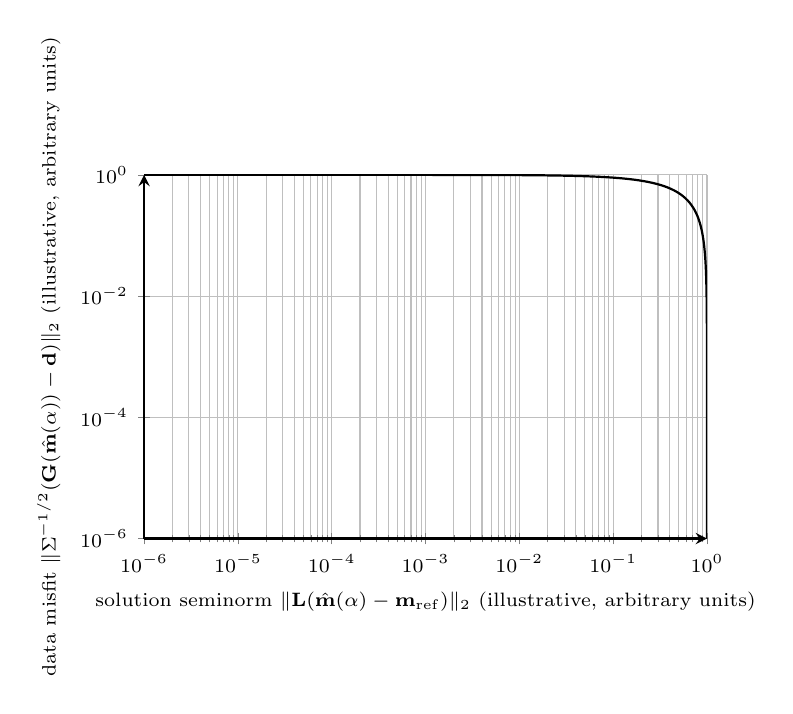
\begin{tikzpicture}
\begin{axis}[
 width=0.72\textwidth,
 height=6.2cm,
 xmode=log, ymode=log,
 xlabel={solution seminorm $\|\mathbf L(\hat{\mathbf m}(\alpha)-\mathbf m_{\mathrm{ref}})\|_{2}$ (illustrative, arbitrary units)},
 ylabel={data misfit $\|\boldsymbol\Sigma^{-1/2}(\mathbf G(\hat{\mathbf m}(\alpha))-\mathbf d)\|_{2}$ (illustrative, arbitrary units)},
 grid=both, axis lines=left, thick,
 label style={font=\scriptsize}, tick label style={font=\scriptsize},
]
\addplot[domain=-3:3,samples=200,black,thick] ({(10^x)^2/((10^x)^2+1)},{1/((10^x)^2+1)});
\end{axis}
\end{tikzpicture}
\caption{Illustrative, schematic L-curve generated from the explicit analytic parametrization $\big(\rho(\alpha),\eta(\alpha)\big)=\big(\alpha^{2}/(\alpha^{2}+1),\,1/(\alpha^{2}+1)\big)$, plotted on logarithmic axes to display the characteristic knee separating the over-smoothed regime (upper left) from the noise-dominated regime (lower right). The curve is a generic mathematical construction used to explain the corner-selection criterion of Stage~5; it does not represent measured or fitted data from any specific inversion.}
\label{ch15-fig:lcurve}
\end{figure}

\subsection{Stage 6 -- Convergence diagnostics and uncertainty quantification}

Convergence is monitored by the KKT residual norm of \cref{eq:kkt1,eq:kkt2}, the relative decrease in $J$, and, once converged, the reduced chi-square $\chi^{2}_{\nu}=2J_{\mathrm{data}}(\hat{\mathbf m})/(q-p)$, near unity for a correctly weighted, non-overfit solution. Where MCMC refines the point estimate, the Gelman--Rubin $\hat R$ statistic and effective sample size provide the acceptance criteria \cite{ref0709,ref0710,ref0727}. The covariance of $\hat{\mathbf m}$ is propagated through the linearization of $\mathcal F$ to give the interval reported for $\hat\Gamma_{E}$,
\begin{equation}
\mathrm{Var}(\hat\Gamma_{E}) \;\approx\; \left(\frac{\partial \mathcal F}{\partial \mathbf m}\right)^{\!\mathsf T}\!\Big[\mathbf J^{\mathsf T}\boldsymbol\Sigma^{-1}\mathbf J + \alpha\mathbf L^{\mathsf T}\mathbf L + \textstyle\sum_{j}\mu_{j}\mathbf D_{j}^{\mathsf T}\mathbf D_{j}\Big]^{-1}\left(\frac{\partial \mathcal F}{\partial \mathbf m}\right) \, , \label{eq:gammaE-variance}
\end{equation}
evaluated at $\hat{\mathbf m}$, the same Gram matrix governing both \cref{eq:gauss-newton} and the stability argument of \cref{sec:pci-objective}.

\section{Assumptions and Their Validation Strategy}
\label{sec:pci-assumptions}

No inversion framework is physics-free, and the credibility of the PCI reconstruction rests on a short list of explicit assumptions, each paired below with a strategy to test rather than merely postulate it. This is deliberately separate from C1--C6: the constraints are relations imposed \emph{within} the estimation, always satisfied at the reconstructed state by construction, whereas the assumptions are conditions under which the entire modelling framework -- choice of forward operators, of which relations qualify as constraints, and of state-space parametrization -- is itself appropriate. A violated constraint shows up as a large residual; a violated assumption is often invisible from within the problem the framework cannot test a premise it was built on.

\begin{enumerate}
\item \textbf{Known atomic/collisional rate data.} $\mathbf G_{\mathrm{OES}}$ needs excitation/de-excitation rate coefficients from an external cross-section database; sensitivity of $\hat{\mathbf m}$ to a bounded perturbation of these is propagated through \cref{eq:gammaE-variance} as an explicit systematic contribution rather than folded into $\boldsymbol\Sigma_{1}$.
\item \textbf{Quasi-one-dimensional sheath geometry.} \Cref{eq:poisson-sheath} assumes a locally planar sheath, tested by comparing chord-averaged interferometry against spatially resolved LIF/OES; where curvature is significant, the framework extends to a 2D-axisymmetric Poisson solve.
\item \textbf{Collisionality regime.} The collisionless/weakly-collisional choice, parametrized by $\mathrm{Kn}_{\mathrm i}$, is validated by a pressure scan (typically \SI{1}{\pascal} to \SI{100}{\pascal}): reconstructed $\mathrm{Kn}_{\mathrm i}$ should track $1/p$ scaling of the mean free path; a systematic departure flags an inadequate closure \cite{ref0077}.
\item \textbf{Steady or periodic-steady operation.} Monitored via residual power in phase bins beyond $N$ and cycle-to-cycle repeatability; a growing high-harmonic residual signals under-resolved nonlinearity or drift requiring the aperiodic formulation.
\item \textbf{Negligible dust/particulate charging and surface contamination.} Checked prior to inversion by independent imaging/process-chemistry evidence; extending C1--C6 to a dusty or electronegative sheath is a model-family choice made upstream, not fitted within the inversion.
\item \textbf{Accurate diagnostic-specific calibration models.} Each $\mathbf G_{j}$ carries instrument constants assumed known independently. Because the problem is over-determined (\cref{sec:pci-overdetermination}), a leave-one-diagnostic-out cross-validation -- refitting from three channels and comparing the withheld channel's prediction to its measurement -- gives an independent test \cite{ref0719}.
\item \textbf{Local linearizability for the Gauss--Newton solver.} Convergence to the global rather than a spurious local minimizer of the non-convex \cref{eq:objective} is not guaranteed a priori; checked via multiple restarts from perturbed $\mathbf m^{(0)}$, agreement with an independent reduced-dimension MCMC exploration, and trust-region step-acceptance monitoring.
\item \textbf{External ground truth.} Where available, $\hat\Gamma_{E}$ is compared against direct, intrusive flux sensors -- dedicated ion-energy-flux sensors \cite{ref0075} and sheath-accelerated secondary-electron flux monitors \cite{ref0078} -- the closest available approximation to independent, non-optical ground truth.
\end{enumerate}

\Cref{tab:assumptions} summarizes this validation matrix.

\begin{table}[htbp]
\centering
\caption{Assumptions underlying the physics-constrained inversion framework and the corresponding validation strategy.}
\label{tab:assumptions}
\begin{tabularx}{\textwidth}{@{}p{4.6cm} X@{}}
\toprule
Assumption & Validation strategy \\
\midrule
Known atomic rate data & Propagate bounded rate-coefficient perturbation through \cref{eq:gammaE-variance} \\
Quasi-1D sheath geometry & Cross-check spatially resolved LIF/OES against chord-averaged interferometry \\
Collisionality regime ($\mathrm{Kn}_{\mathrm i}$) & Pressure scan; test $1/p$ scaling of inferred mean free path \\
Periodic-steady operation & Monitor high-harmonic residual and cycle-to-cycle repeatability \\
No dust/electronegative contamination & Independent process/imaging evidence prior to inversion \\
Diagnostic calibration models & Leave-one-diagnostic-out cross-validation \\
Local linearizability of solver & Multi-restart agreement; reduced-dimension MCMC cross-check \\
Overall pipeline & Comparison against intrusive flux sensors where available \\
\bottomrule
\end{tabularx}
\end{table}

\section{Summary}
\label{sec:pci-summary}

This chapter formalized reconstruction of $\GammaE$ as a single constrained nonlinear estimation problem over a shared plasma/sheath state $\mathbf m$, rather than four sequential, individually ill-posed deconvolutions. The forward model of \cref{sec:pci-forward} showed the four channels probe complementary projections of $\mathbf m$: no single Jacobian block has full column rank, but the stacked, physics-augmented Jacobian generically does. The regularized objective of \cref{sec:pci-objective} makes this over-determination operationally useful, with well-posedness restored by the combined action of a generic prior and the physically motivated constraints; the time-resolved extension of \cref{sec:pci-time} carries the same architecture into RF-periodic and transient regimes where $\GammaE(t)$, not a single number, is the physically meaningful target. The pipeline of \cref{sec:pci-algorithm} and the assumption inventory of \cref{sec:pci-assumptions} are integral to this claim of well-posedness: an inversion that cannot state, test, and revise its own assumptions is not more trustworthy than the single-diagnostic fits it replaces, merely more elaborate.

The central innovation of PCI, and why it is a distinct contribution rather than a routine application of existing IDA machinery \cite{ref0707,ref0712,ref0727}, is its choice of regularizer: rather than a generic smoothness or maximum-entropy prior, it uses the kinetic Bohm criterion, the sheath Poisson/Child--Langmuir relation, and particle- and energy-flux continuity of the plasma--sheath transition itself -- the same conservation and boundary-layer relations developed from first principles earlier in this monograph. Their use as \emph{active constraints inside the estimation}, rather than as passive post-hoc checks, is what converts four separately under-determined optical inversions into one jointly well-posed estimate of $\GammaE$ with quantified, physically defensible uncertainty -- a property the remaining chapters build upon in applying the framework to electric propulsion, plasma etching, and fusion plasma-facing-component contexts. Because PCI treats each of C1--C6 as an auditable residual rather than an implicit assumption baked into a black-box estimator, the reconstructed $\hat{\mathbf m}$ carries a transparent record of which physical relations filled in what the four channels alone could not determine, and by how much each moved the estimate from the raw, unconstrained fit -- the traceability later chapters rely upon in specifying the experimental campaign, uncertainty budget, and validation plan needed to take PCI from algorithmic construction to a demonstrated, defensible measurement of ion energy flux across a real plasma sheath.
